\chapter{UI/UX Design}\label{chapter:ui_ux_design_reqs}

\begin{chapterabstract}
    This chapter explains the reasoning behind some of the core design decisions, 
    specifies the software requirements, 
    and provides an overview of the GUI layout.
\end{chapterabstract}

\section{Real-time approach}
Ambilink's\footnote{``Ambilink'' is the name given to the software during early stages of development.} main goal lies in allowing to utilise animation data 
from a Blender scene for ambisonic panning in a DAW. This is achieved with a pair of plugins - a Blender plugin and a VST plugin.
The Blender plugin (or ``add-on'', using Blender's official terminology) 
provides data about the 3D scene to instances of the VST plugin, that perform the ambisonic panning.
Deciding how this data will be passed from the Blender add-on to the VST was the earliest design decision that had to be made, 
since the chosen approach would dramatically affect the way the software functions, and, naturally, the user experience. 

One solution would be to export animation data from Blender to a file.
The data could then be imported by the VST plugin.
Unfortunately, such a solution, although simple to implement, would be quite suboptimal from a UX perspective.
Music production experience has taught me that immediate feedback is immensely helpful when making creative decisions, 
and that decisions made by sound designers and mixing engineers are undoubtedly of creative nature.
Thus, from the very beginning, I've designed the software to include real-time preview functionality - 
the panning directions are continuously updated based on the current state of the Blender scene, 
allowing the user to immediately hear how adjustments performed in Blender affect the audio mix.

Of course, the real-time approach also has it's downsides. It increases the overall complexity of the system,
and may introduce new types of problems stemming from connection issues. 
Communication latency may also negatively affect responsiveness.
A good implementation should however be able to avoid or mitigate these flaws.

\section{Requirement definition}
Once the decision to make the system real-time was made, I've settled on some functional and non-functional requirements to guide the development.
\subsection*{Functional requirements}
\begin{funcreqs}
    \item The system consists of two components - the Blender add-on and the VST plugin.
    \item The user is able to pick an object from the Blender scene using the VST plugin.
    The location of that object is then used to calculate the panning direction used by the VST plugin.
    \item Whenever the location of a Blender object is updated (manually or during animation playback), 
    the panning directions are updated in real time. (Communication between the two components is performed in real time.)
    \item When a VST instance is bound (subscribed) to a specific Blender object, renaming or deleting the object in Blender is reflected by the VST GUI.
    \item The VST plugin supports offline rendering\footnote{Offline rendering refers to exporting the audio, as opposed to real-time (online) playback during the production process.}.
    The exported audio is synchronised to the animation.
    \item The distance from a Blender object to the camera affects the gain of the respective VST distance; 
    the user is able to choose from multiple distance attenuation models.
    \item The user is able to pick the Ambisonics order and normalisation type (N3D or SN3D) used by the plugin.
\end{funcreqs}

\subsection*{Non-functional requirements}
It has to be noted that since the software can run on any number of hardware configurations,
it is hard to define performance-related requirements unambiguously. 
Thus, the ``scales well'' formulation used in the non-functional requirements below
should be understood as ``scales well for the hardware''.

\begin{nonfuncreqs}
    \item Selecting an object from the Blender scene via the VST GUI is quick,
    even when the scene contains a large number of objects.
    \item Real-time direction updates have an acceptable delay, ideally less than 0.5 seconds.
    \item The system scales well for Blender scenes containing a large number of objects (e.g. thousands). 
\end{nonfuncreqs}

\section{User interaction}
% Suggested: nejaky use-case diagram?? -> Would not bring value, single actor, single use case, functional requirements specified differently
With the requirements in place, the next step was designing the way the user will interact with the software.
In case of Ambilink, this was a relatively straightforward process, 
since the system has a single use case, that only requires limited user interaction.
A user's workflow might roughly follow these steps:
\begin{enumerate}
    \item Open the Blender project, and start the Ambilink Blender add-on.
    \item Open the DAW, and place the Ambilink VST on the channels containing sounds that should correspond to objects in the Blender scene.
    \item For each instance of the Ambilink VST, select an object from the Blender scene.
    \item Adjust ambisonics-related settings (order, normalisation type) to match what's being used in the project.
    % //TODO: if there's time and it's easy to implement, store these "global" settings in a config file. Otherwise, add a note about this being a limitation of the current version.
    \item Make any necessary adjustments to the Blender scene, or the audio mix, including adjusting distance attenuation parameters of the Ambilink VST.
    \item Render the resulting audio.
\end{enumerate}

\subsection{Blender add-on}
The Blender plugin needs to support two main actions - launching and stopping the server that will provide data to the VSTs.
Most operations in Blender are realised using so-called operators that essentially encapsulate any action that can be performed by the user.
Operators can be invoked via buttons in the GUI or using Blender's search functionality.
Because the user shouldn't have to start or stop the server often, I've chosen to avoid adding an additional panel to the GUI.
Instead both actions are realised using operators that can be invoked from the \cppinline{File > Export} menu, or using search.

The Blender add-on depends on an external Python module.\footnote{External dependencies will be discussed in Chapter \ref{chapter:implementation}.}
I did not want to include the module's code as part of the addon, or to automatically install third-party modules without informing the user.
Instead I've chosen to be transparent and require the user to explicitly initiate dependency installation.
This can be done by pressing a button in Ambilink's add-on preferences panel which can be accessed through Blender's preferences dialogue.
If dependencies aren't installed and the user invokes the ``Start Server For Ambilink VST'' operator,
an error message is shown that instructs the user to install dependencies via add-on settings.

\subsection{VST plugin}

The VST plugin should allow the user to perform a much wider range of actions - selecting an object from the Blender scene, changing distance attenuation and ambisonics parameters.
Figure \ref{fig:gui_prototype} shows a wireframe of the user interface created before implementation.
The GUI consists of a main screen that is shown at launch and two additional screens - the object selection screen and the settings screen.

\paragraph*{Main screen}
The main screen displays the currently active object (if any), and a visual indicator of the current direction from the camera to the object.
It also allows to adjust the distance attenuation type and maximum distance to the camera at which the sound gain will be above 0 dB.
The distance attenuation parameters are located on the main screen to minimise the number of clicks required to adjust them. 
This is done because various sounds may require different values, 
depending on the distance at which the user would want them to become audible.
By pressing the button on the right side of the active object indicator the user can transition to the object selection screen.
The settings screen can be accessed by pressing the ``Settings'' button located in the top right corner of the UI.

\paragraph*{Object selection screen}
The object selection screen allows the user to select an object from the Blender scene. Since the Blender scene may include a 
high number of objects, a search box is present in the top part of the UI, allowing the user to quickly find a specific object.
When searching, the first object in the list is highlighted; the user can then select that object by pressing the ``Enter'' key.

\paragraph*{Settings screen}
The settings screen is reserved for plugin parameters that are not expected to be adjusted often,
and can thus be placed on a separate screen to avoid cluttering the main UI (and save space for adding new parameters further down the line).
Right now it only includes the ambisonics order and the normalisation method.
The user should only need to adjust these parameters once per project most of the time.

\begin{figure}    
    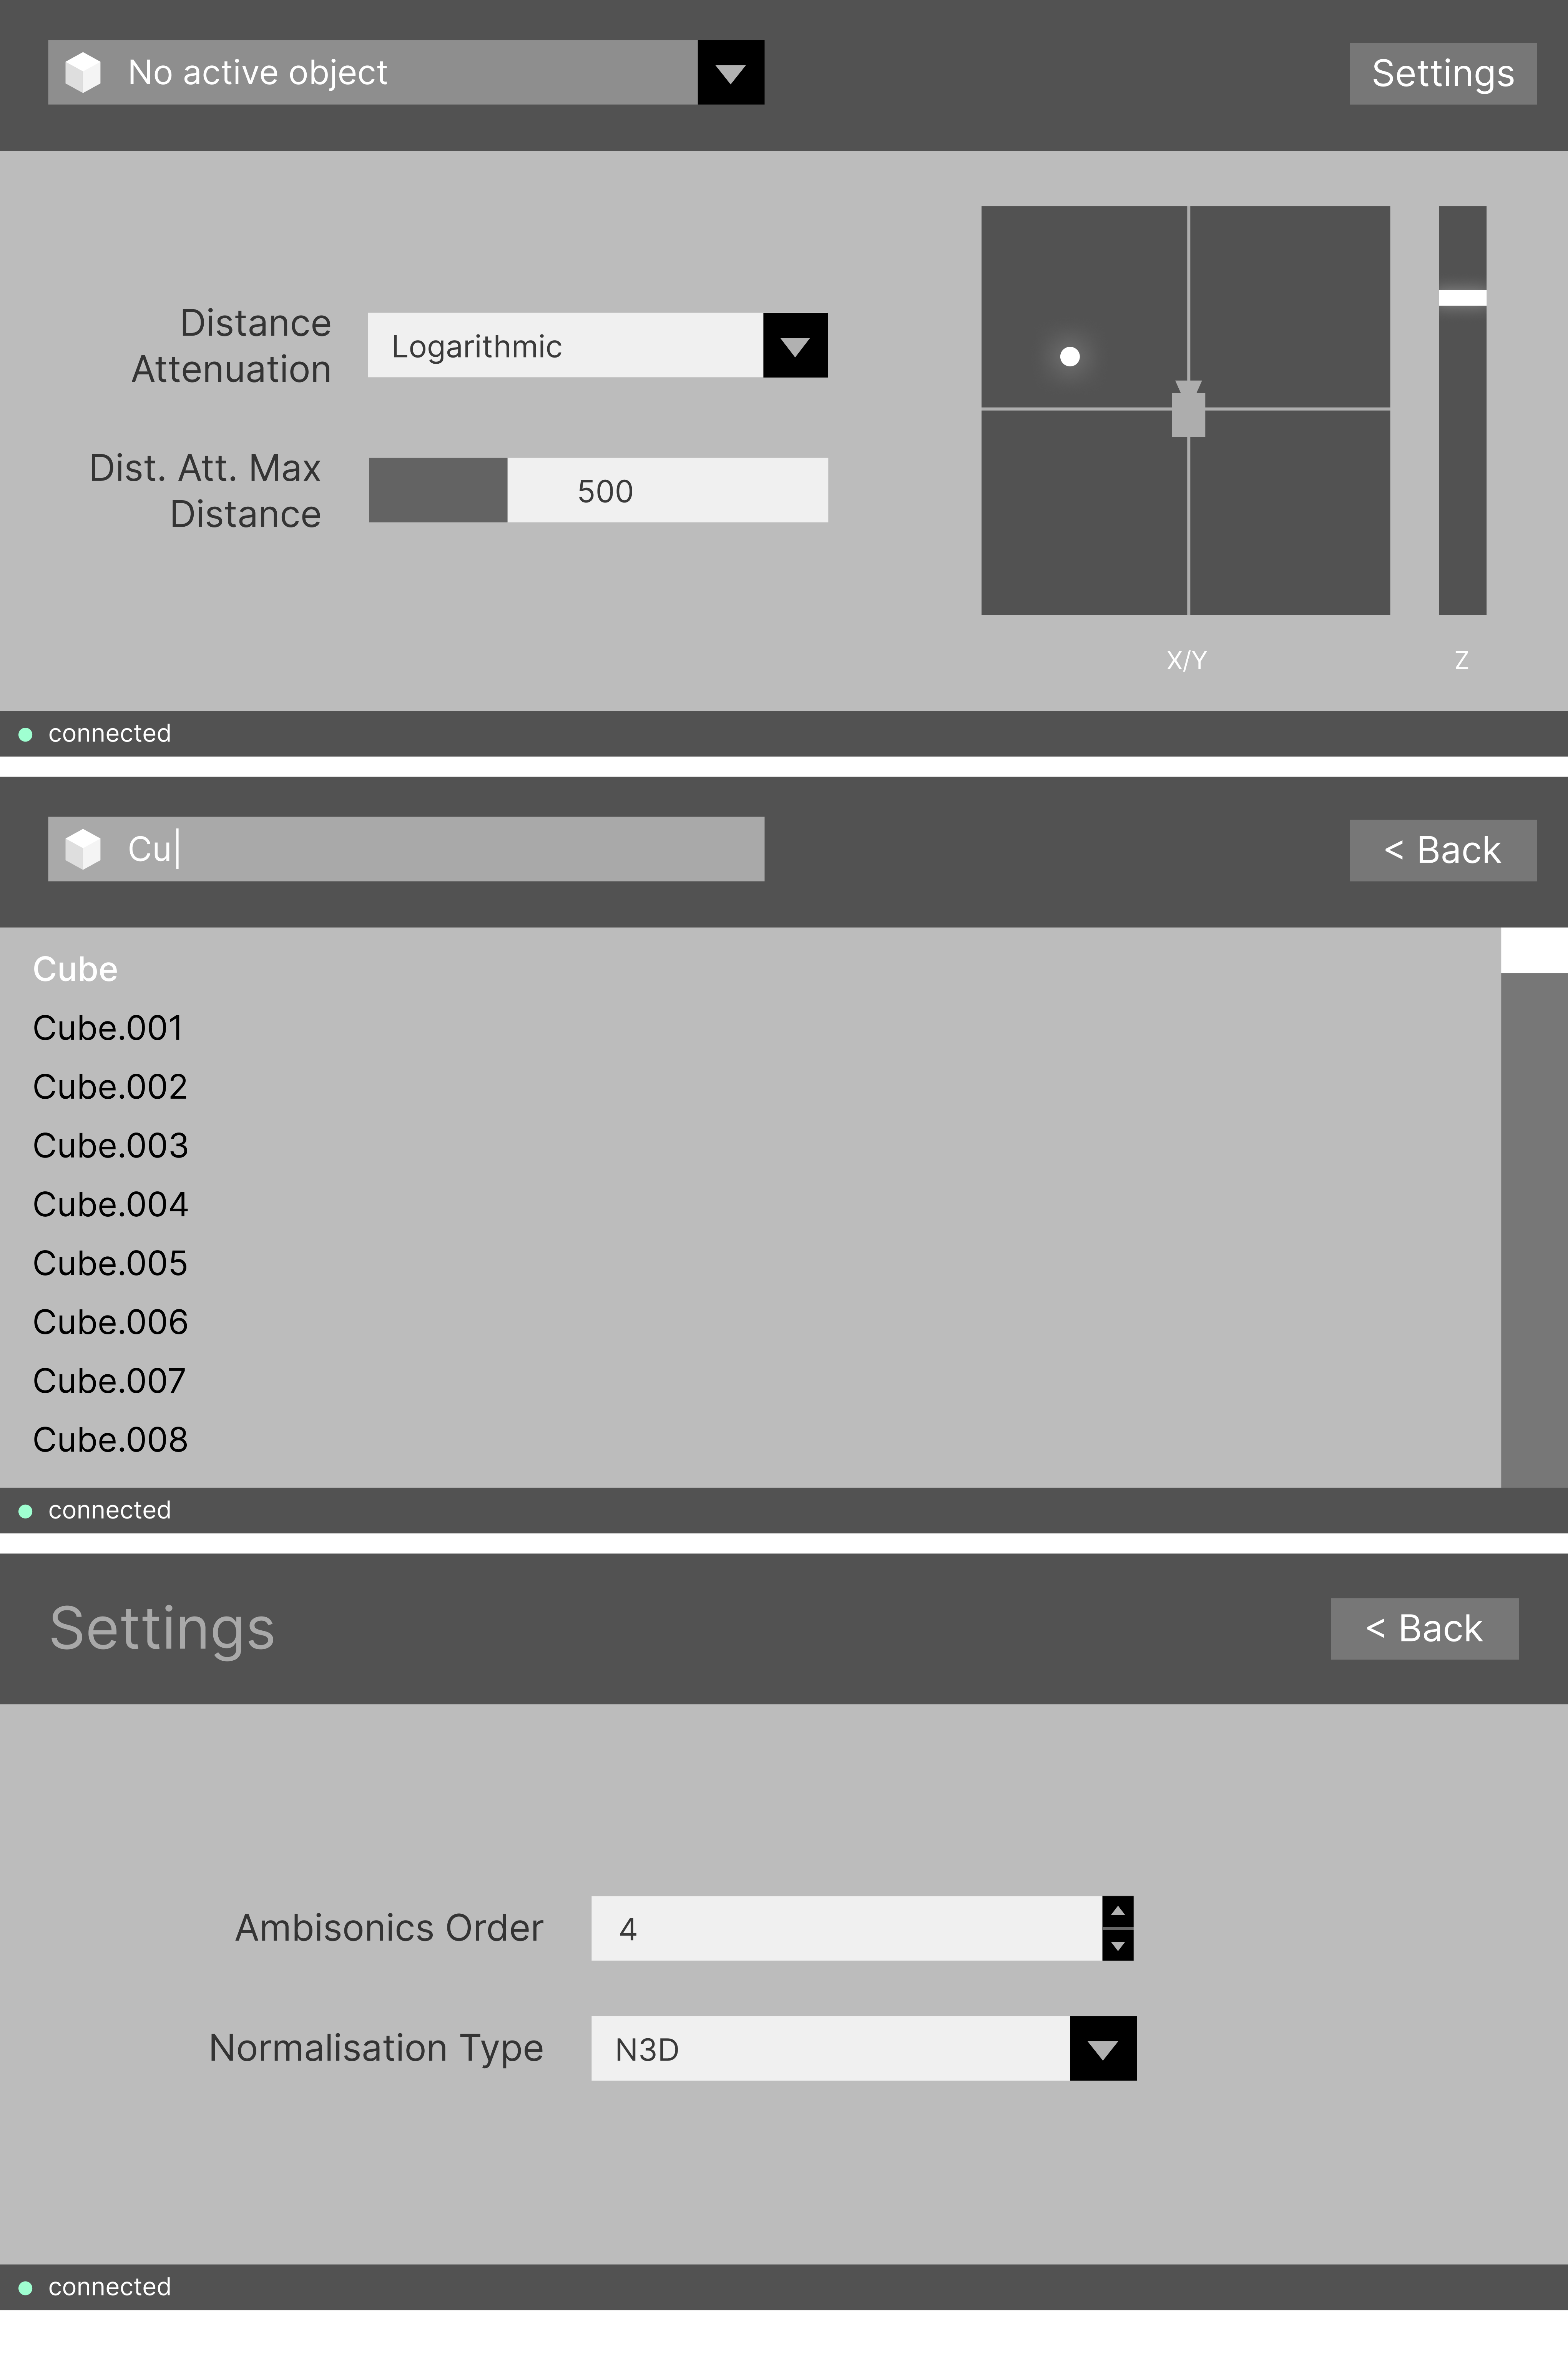
\includegraphics[width=0.9\textwidth]{images/implementation/gui_wireframe_whitespace_bottom.png}
    \centering
    \caption{Prototype GUI layout for the VST plugin. From top to bottom: main screen, object selection screen, settings screen.
             Image courtesy of the author. \label{fig:gui_prototype}}
\end{figure}

% ===========================================================
% ===================== IMPLEMENTATION ======================
% ===========================================================
% - IPC Communication Overview (mentions NNG, and it's role)
% - VST Plugin
%   - Technologies Used
%   - High level structural overview
%   - IPC Client
%   - Encoder
%   - Passing data lock-free (prilohy)
% - Blender Plugin
%   - Technologies Used
%   - Structural overview
%   - Overcoming Blender API Limitations (prilohy)

\chapter{Implementation}\label{chapter:implementation}

\begin{chapterabstract}
    This chapter provides an overview of the implementation of the Blender add-on and the VST plugin.
    It present the structure of the IPC protocol, describes the top level architecture of each component, 
    and provides some insight into the challenges that had to be solved.
\end{chapterabstract}

\begin{figure}[!h]
    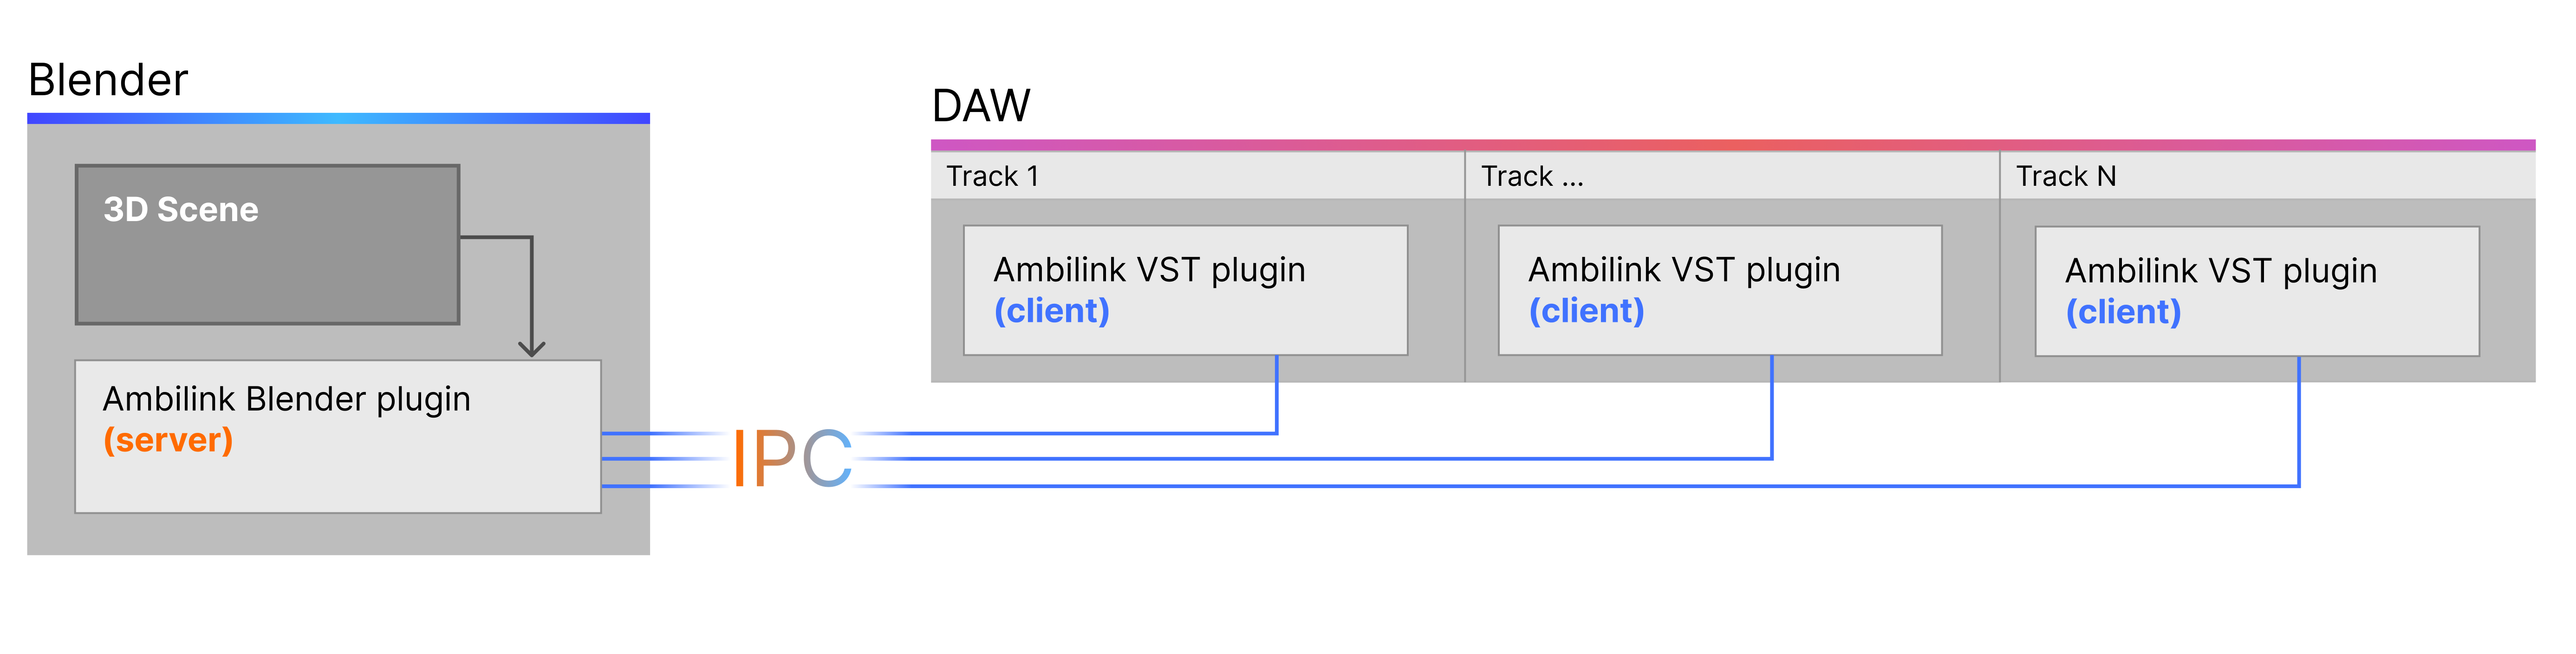
\includegraphics[width=\textwidth]{images/implementation/plugin_interaction_diagram.png}
    \caption{Diagram of high level interaction between the VST instances and the Blender plugin.
        Image courtesy of the author. \label{fig:component_diagram}}
\end{figure}

\section{IPC Protocol}
To minimise latency in communication between the Blender add-on and the VST plugin, Ambilink utilises IPC
\footnote{IPC is a generic term - interprocess communication may very well be realised using TCP or other network protocols.
In the context of this thesis, however, the term IPC is used to refer to any form of ``direct'' interprocess communication, such as named pipes or shared memory.}.
Since Ambilink is developed in a way that should enable eventual support of all three major operating systems,
utilising OS-specific IPC mechanisms directly was undesirable.
Instead, I've chosen to entrust the low level details of interprocess communication to a third-party library - NNG (nanomsg-next-gen).
NNG is multiplatform, provides support for various transports (e.g. IPC, TCP, WebSockets), as well as common communication patterns (e.g. Request/Response, Publisher/Subscriber).
While NNG itself is written in C, wrappers exist for many popular programming languages, including Pynng for Python, as well as nngpp for C++.
(The latter serves more as a quality of life improvement, as NNG's C interface can of course be used directly from C++ code.)
Using the library also highly increases flexibility of the implementation, allowing, for example, to replace IPC with network communication via TCP or WebSockets with minimal effort.
All of this made NNG a great choice for Ambilink.

Figure \ref{fig:component_diagram} illustrates how the individual components are connected via IPC from a high level perspective.
The Blender plugin takes on the role of a server, providing information about the Blender scene to
an arbitrary number of clients - instances of the VST plugin. 

\begin{figure}
    \centering
    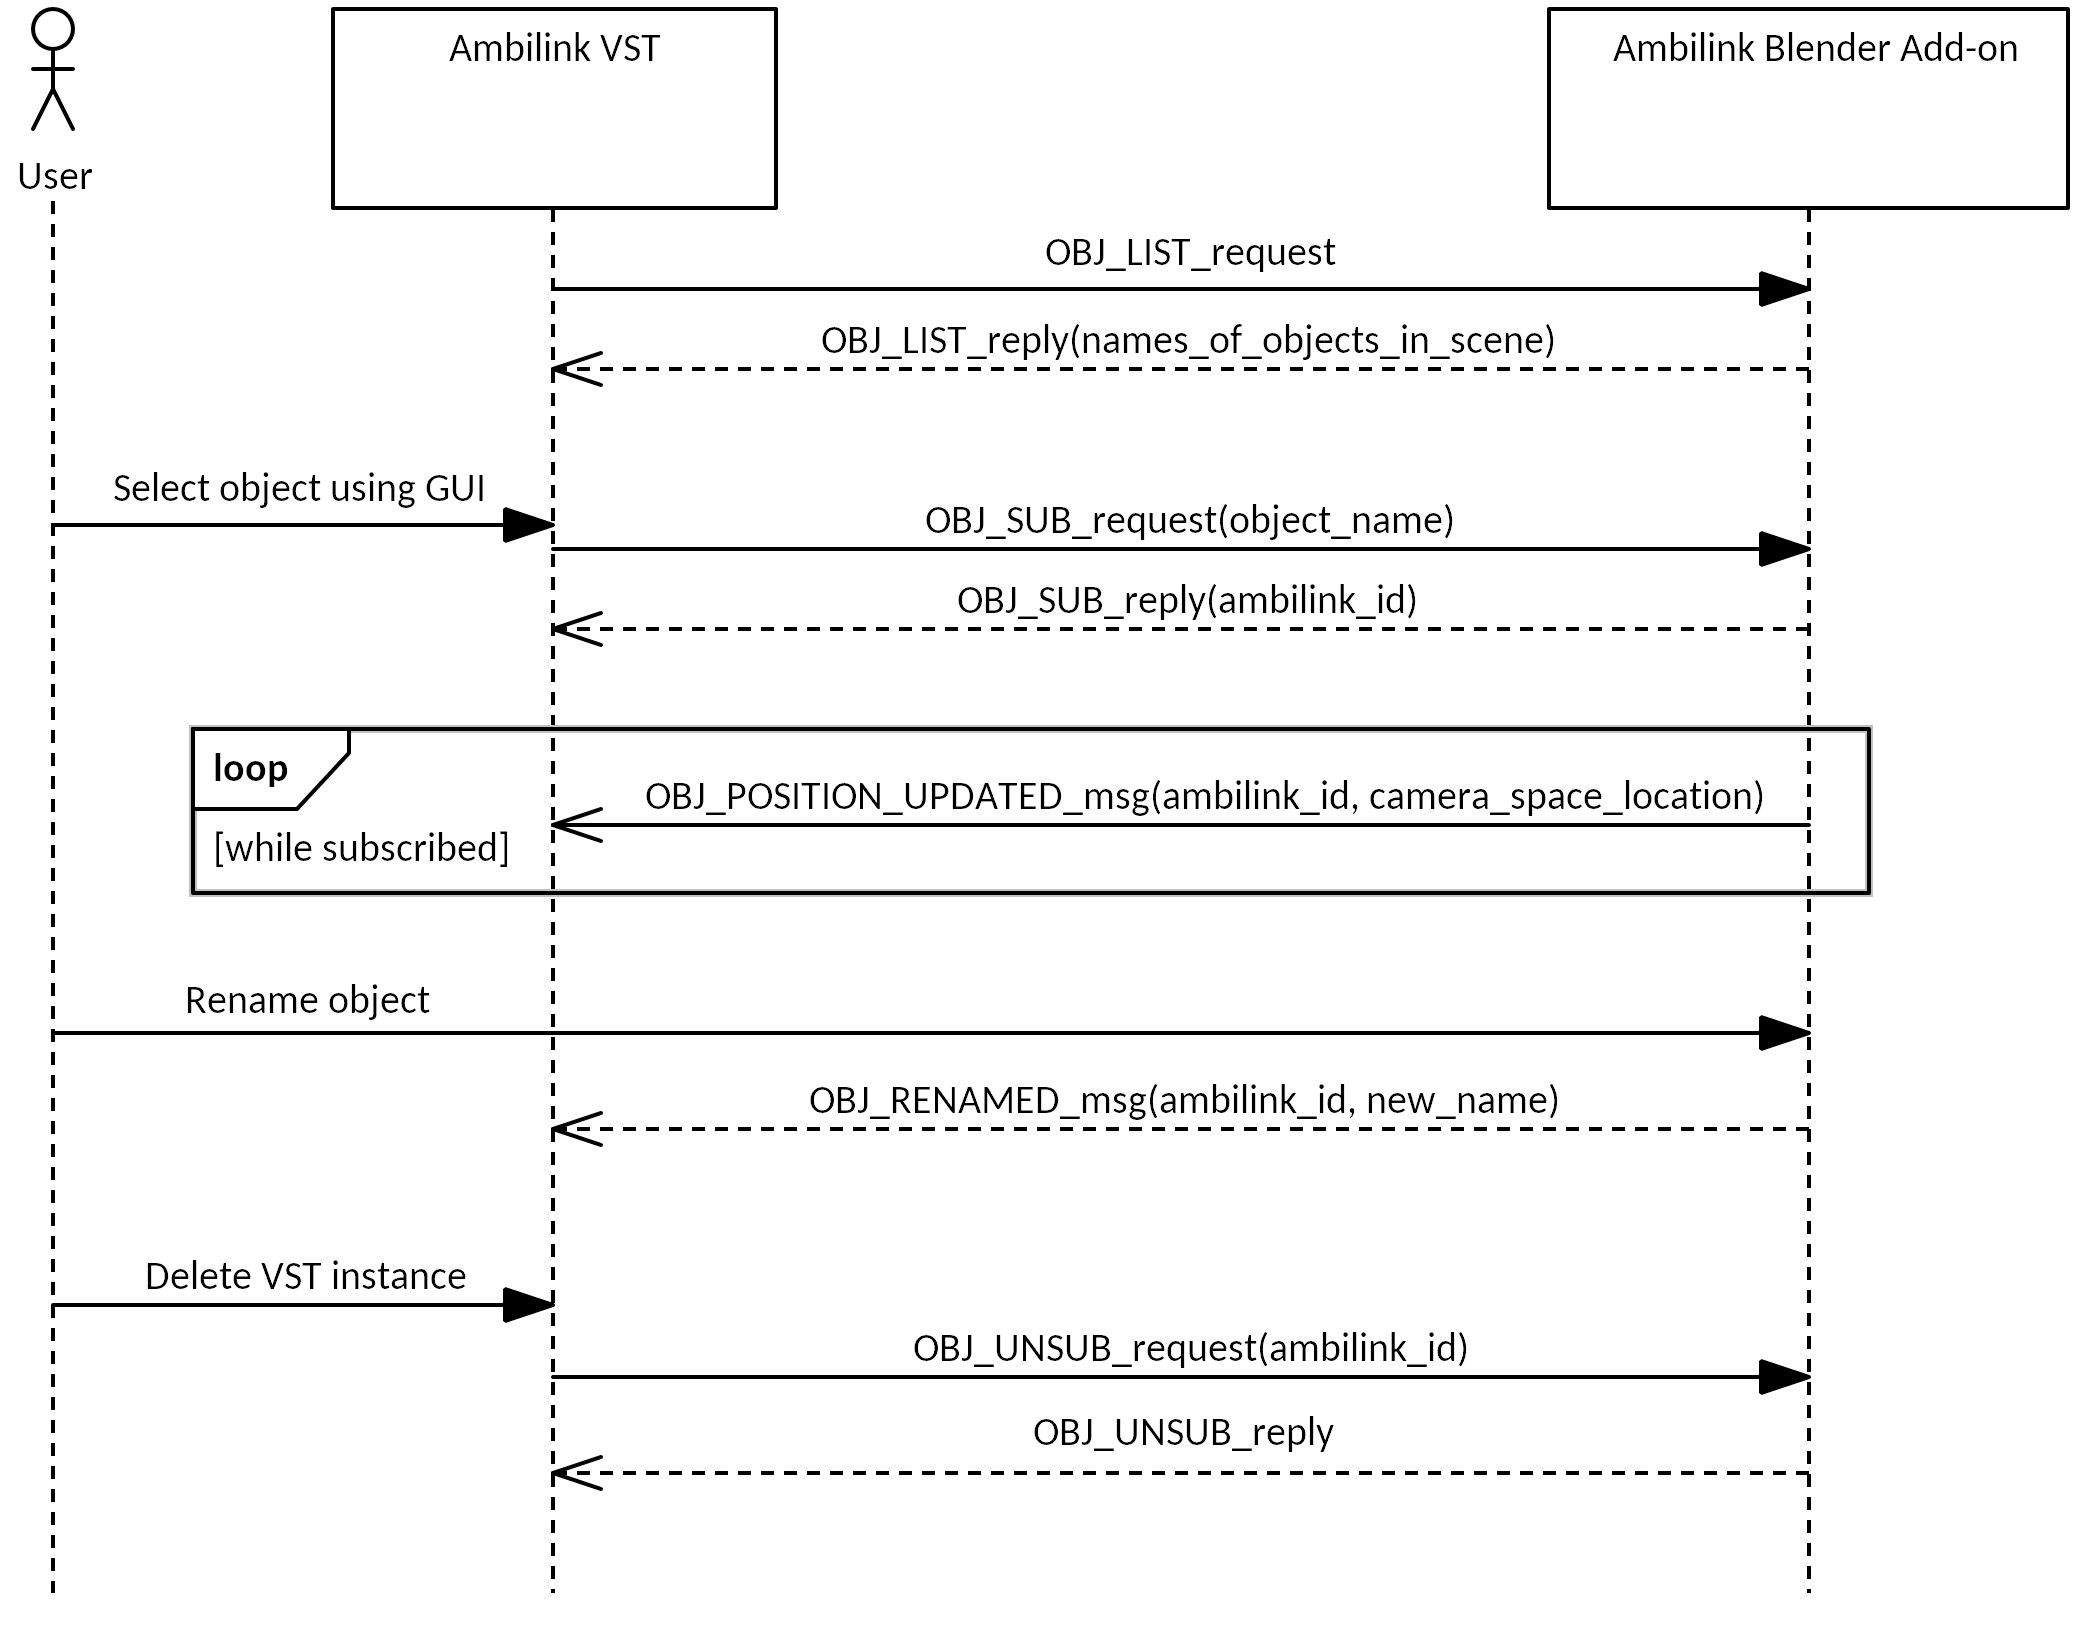
\includegraphics[width=0.95\textwidth]{images/implementation/basic_comm_sequence.png}
    \caption{Communication sequence between the Blender plugin and an instance of the VST plugin during real-time (online) rendering.
             Messages with the suffix ``request'' or ``reply'' are sent using Req/Rep.
             Messages with the suffix ``msg'' are sent using Pub/Sub.
             Image courtesy of the author. \label{fig:basic_comm_sequence}}
\end{figure}

A sequence diagram illustrating communication between the two plugins in real-time rendering mode is shown in figure \ref{fig:basic_comm_sequence}.
First, the user picks an object from the Blender scene. The VST instance then subscribes to that object,
requesting the Blender add-on to begin informing it about updates to the object's location and other important events.
The object is then renamed in Blender, and a rename notification is published by the Blender add-on, allowing the VST GUI to update the object name.
Finally, the VST instance is deleted by the user; it's destructor sends a request to unsubscribe from the object. 
(Object position updates would have continued after the rename message if the instance hadn't been destroyed.)
Two different communication patterns implemented by the NNG library were used during that sequence:
\begin{description}
    \item[Request/Reply (Req/Rep)] This pattern is used for all communication initiated by the VST instance - requesting the list of objects in the Blender scene, subscribing to an object, 
    requesting object location data for offline rendering, etc.
    \item[Publisher/Subscriber (Pub/Sub)] In this pattern, a single publisher produces messages that are consumed by multiple subscribers.
    Ambilink starts using this pattern once a VST instance is subscribed to an object. The Blender plugin serves as the publisher, and the VST plugin instances as the subscribers.
    Messages published by the Blender plugin include object location updates (published multiple times per second for all objects with at least one subscribed VST instance),
    object name updates, and object deletion notifications.
\end{description}

\subsection{Protocol messages}
\begin{listing}[ht]
    \begin{minted}{python}
    class ReqRepCommand(IntEnum):
        OBJ_LIST = 0x01
        OBJ_SUB = 0x02
        OBJ_UNSUB = 0x03
        PREPARE_TO_RENDER = 0x04
        INFORM_RENDER_FINISHED = 0x05
        GET_RENDERING_LOCATION_DATA = 0x06
        GET_ANIMATION_INFO = 0x07
        PING = 0xFF
    
    class ReqRepStatusCode(IntEnum):
        SUCCESS = 0x00
        OBJECT_NOT_FOUND = 0x01
        INVALID_REQUEST_DATA = 0x02
        INTERNAL_ERROR = 0xFE
        UNKNOWN_COMMAND = 0xFF
    \end{minted}
    \caption{Definition of IPC protocol constants used in Req/Rep messages. (From the source code of the Blender add-on.)}
    \label{code:ipc_constant_definition}
\end{listing}

This section provides an overview of the message structure for each communication patter used in the IPC protocol. 
The \cppinline{documentation/ipc.md} file included on the attached media defines the structure of 
each individual message type. Alternatively, documentation generated using Doxygen (\cppinline{documentation/Doxyfile} on the attached media) 
will also include the contents of the file.

\paragraph*{Request/Reply}
The Request/Reply part of the  protocol consists of a set of commands differentiated by a single-byte command code.
A request always starts with the command code, and a reply starts with a status code (also a single byte) indicating if the operation was successful
or the reason it failed. In both cases optional command-specific data may follow. 
Listing \ref{code:ipc_constant_definition} shows the list of all commands and status codes and the corresponding constants.

\paragraph*{Ambilink IDs}
During the initial stage of communication (before a subscription is established) Blender objects are referenced by their name.
While object names in Blender are unique, using the object's name as the identifier would not be viable as the objects 
can be renamed after the subscription is established.
It would also be inefficient - a whole string would have to be passed for every request referencing a specific object,
as well as in every message published by the Blender add-on, increasing the size of most messages.
Because of these factors, once a subscription is established, a unique numeric identifier is used to reference Blender objects.
This value, called an Ambilink ID, is assigned by the Blender plugin
\footnote{The process of Ambilink ID assignment will be discussed in more detail in \ref{subsection:blender_api_fun}.},
and returned as part of the reply to an \cppinline{OBJ_SUB} request.

\paragraph*{Publisher/Subscriber}
Messages published by the Blender add-on start with the AmbilinkID of the object they relate to.
This allows each VST instance to filter out irrelevant messages based on the first two bytes.
After the Ambilink ID, a single-byte message type identifier follows. The Blender add-on publishes the following message types:
\cppinline{OBJ_POSITION_UPDATED}, \cppinline{OBJ_RENAMED}, \cppinline{OBJ_DELETED}. 
\cppinline{OBJ_POSITION_UPDATED} messages include the location of the object in camera space. 
Using camera space coordinates allows to reduce the bandwidth consumed by these messages 
since only one set of coordinates needs to be transmitted. The direction and distance from the object
to the camera are then calculated by the VST plugin.

\subsection{Offline rendering}

\begin{figure}
    \centering
    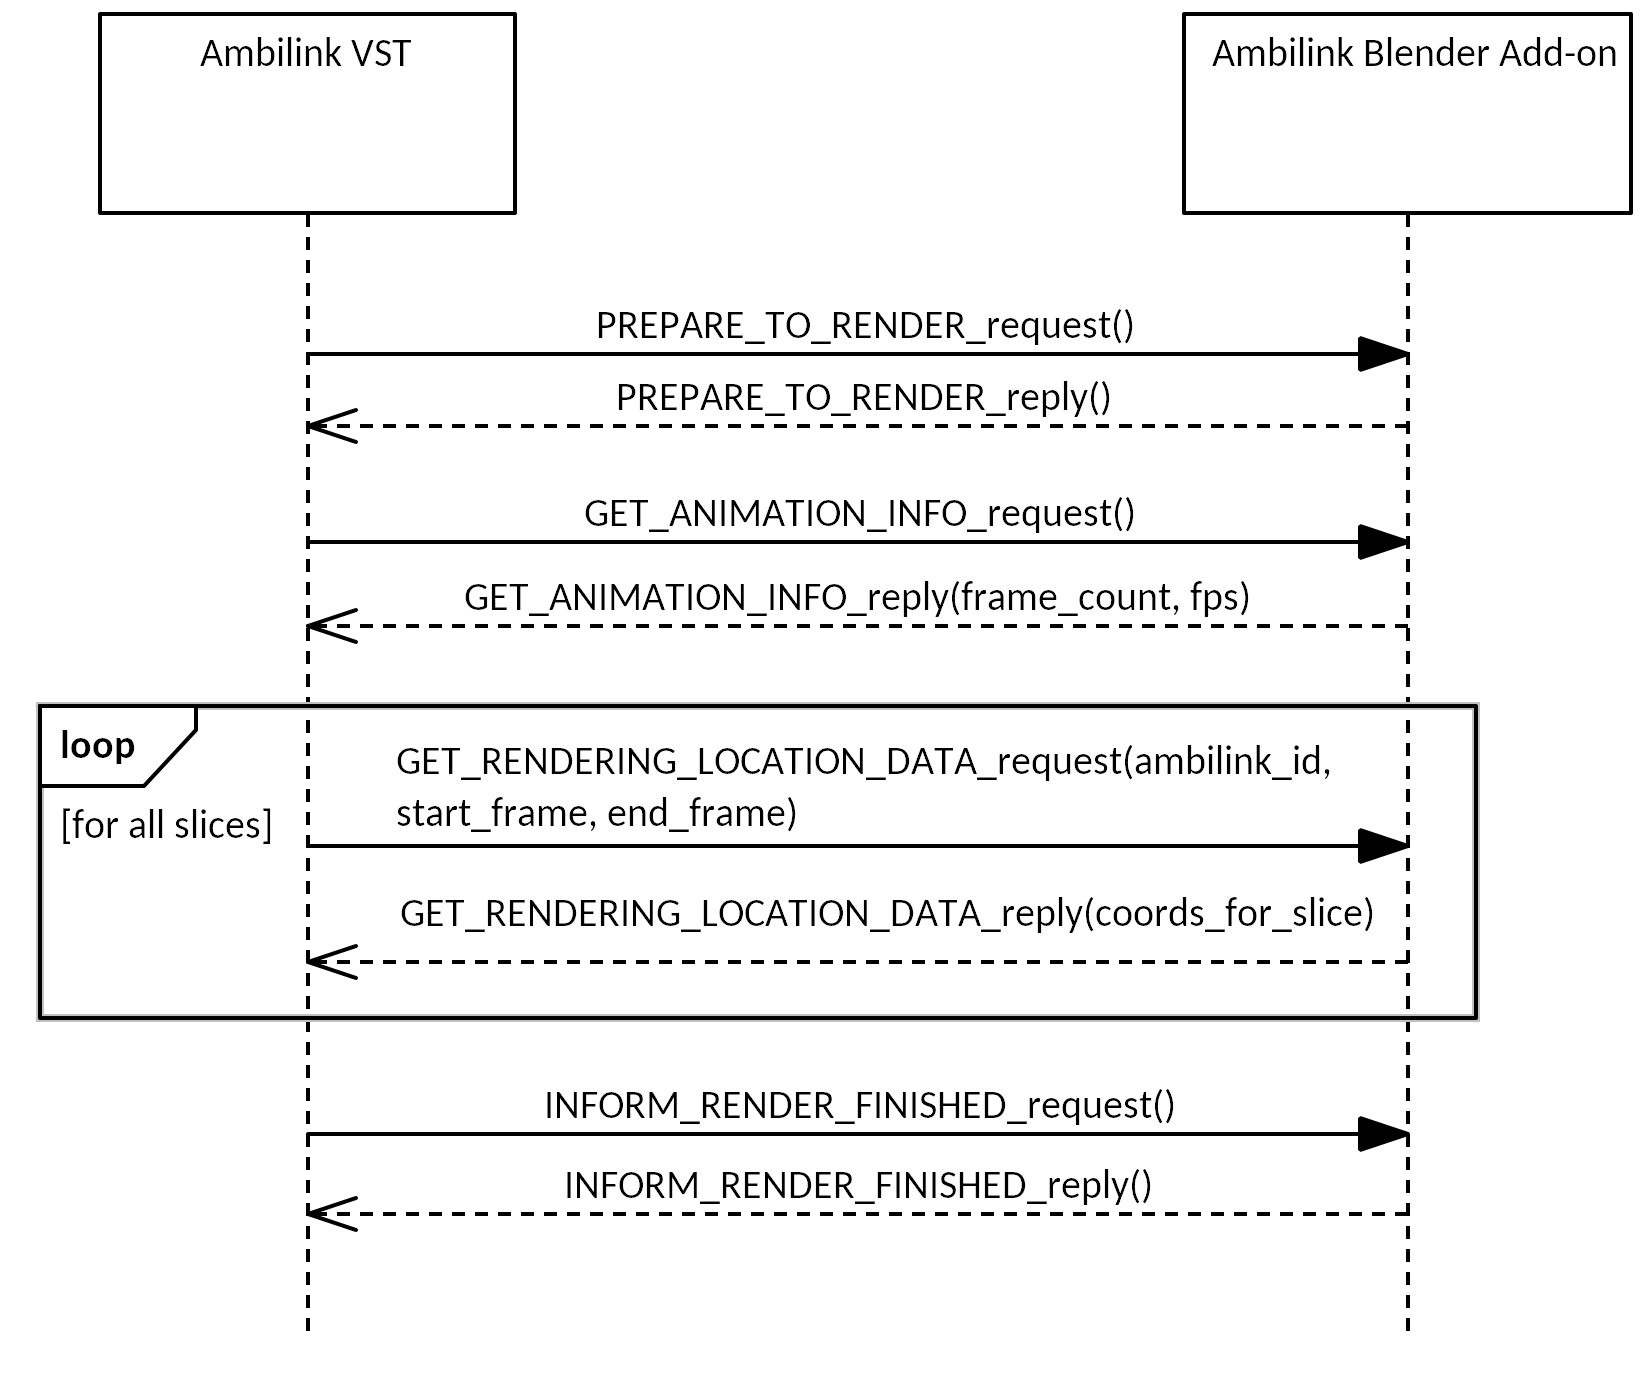
\includegraphics[width=0.9\textwidth]{images/implementation/offline_render_comm_sequence.png}
    \caption{Sequence diagram illustrating communication in offline rendering mode.
             Image courtesy of the author. \label{fig:render_comm_sequence}}
\end{figure}

As can be seen from the sequence diagram in figure~\ref{fig:render_comm_sequence}, 
communication during offline rendering (when the audio is being rendered to a file) significantly differs from communication during real-time playback.
Pub/Sub is not used, instead, every interaction is initiated by the VST.
The \cppinline{PREPARE_TO_RENDER} request includes no additional data and serves as a notification for the Blender plugin 
that a render is about to begin. The Blender plugin will receive this message from each VST instance,
but only the first one will have an effect. While this may seem wasteful, it greatly simplifies the protocol.
Otherwise, all the VST instances would have to communicate with each other, agreeing on a single ``master'' instance.
Once a \cppinline{PREPARE_TO_RENDER} message is received, the Blender plugins stops publishing \cppinline{OBJ_POSITION_UPDATED} messages until the render ends, and invalidates
the cache used during the previous offline render.

To render the audio, a VST instance needs to know the object's camera space coordinates at each frame of the animation.
Instead of requesting all the animation data at once, the VSTs first request the number of frames and FPS of the animation, 
and then get the data in slices using multiple \cppinline{GET_RENDERING_LOCATION_DATA} requests.
(Denoted in fig. \ref{fig:render_comm_sequence} by the ``loop'' fragment.)
This is done because the DAW's GUI thread might be blocked until the first audio sample buffer is processed.
\footnote{This is the case for at least one DAW - Reaper.}
Since Ambilink would not have been able to process the first buffer until all the rendering data is received,
such an implementation would have made the GUI of some DAW's unresponsive for unacceptable periods
when entering rendering mode. Getting rendering data in slices also allows audio processing and IPC to be performed in parallel.

Because the animation may be very long, there is a limit to the number of slices held in memory by each VST instance.
If the memory limit is reached, the VST instance waits for the audio thread to consume the previous slice 
of location data before fetching the next one.

\section{VST plugin}\label{section:vst}
The Ambilink audio plugin is developed in C++ using the JUCE framework and targets Steinberg's VST3 interface\footnote{
    Since VST3 is the only version of the interface that is currently supported by Steinberg,
    I've been mostly referring to it as ``VST'' up to this point and will continue to do so
    unless differences between versions of the standard are discussed.
}. It outputs ambisonics up to fifth order
(The reasons behind this limitation are described in \ref{subsection:vst_limitations}.)
with ACN channel ordering and N3D or SN3D normalisation (configurable via the settings screen).
The code base is multiplatform, but, at the time of writing this thesis, the build system is only operational on Linux.
Documentation comments are used throughout the code base; documentation can be generated using Doxygen 
(see \cppinline{documentation/Doxyfile} on attached media).

\subsection{Third-party libraries}
While developing a VST plugin without a specialised framework is possible, it is highly time consuming,
and takes a lot of ``reinventing the wheel'', that's why Ambilink uses JUCE.
It provides all of the base functionality required for building audio plugins
- a relatively convenient wrapper on top of the base VST interface, a GUI system,
 audio processing primitives, as well as other features not as pertinent to this specific project.
Developing the Ambilink VST with JUCE also opens the opportunity to provide the plugin in other formats 
later on without requiring major changes to the codebase.
Another important factor is that the JUCE framework has a large user base, increasing the number
and availability of learning resources, which was of great help, since I had no prior experience developing audio processing plugins.
Finally, it is dual-licensed under GPLv3 and a proprietary commercial license,
enabling it's use in this project. Besides JUCE, the VST plugin component also uses the Spatial Audio Framework (\cite{saf_repo}) to calculate the spherical harmonics coefficients for a given direction of sound,
as well as vector data types and some useful trigonometric functions from GLM (\cite{glm_repo}).

\subsection{Software architecture}
An audio plugin written with JUCE consists of two main parts. An \cppinline{AudioProcessor} class 
deriving from the \cppinline{juce::AudioProcessor} virtual base class that performs the actual audio processing,
receives audio, MIDI, and other data from the host software. 
The plugin's GUI is implemented in the \cppinline{AudioProcessorEditor}
class that derives from \cppinline{juce::AudioProcessorEditor}.
An instance of the \cppinline{AudioProcessor} class always exists while the plugin is loaded.
\cppinline{AudioProcessorEditor}, on the other hand, is only instantiated once the plugin's GUI editor is open, and is
usually\footnote{Such details may differ between different DAWs.}
destroyed as soon as it is closed.\footnote{A VST plugin does not require a custom GUI, DAW's implement a default GUI for the various audio parameters defined by the VST interface. This was not a viable option for Ambilink.}

\begin{figure}%[!ht]
    \centering
    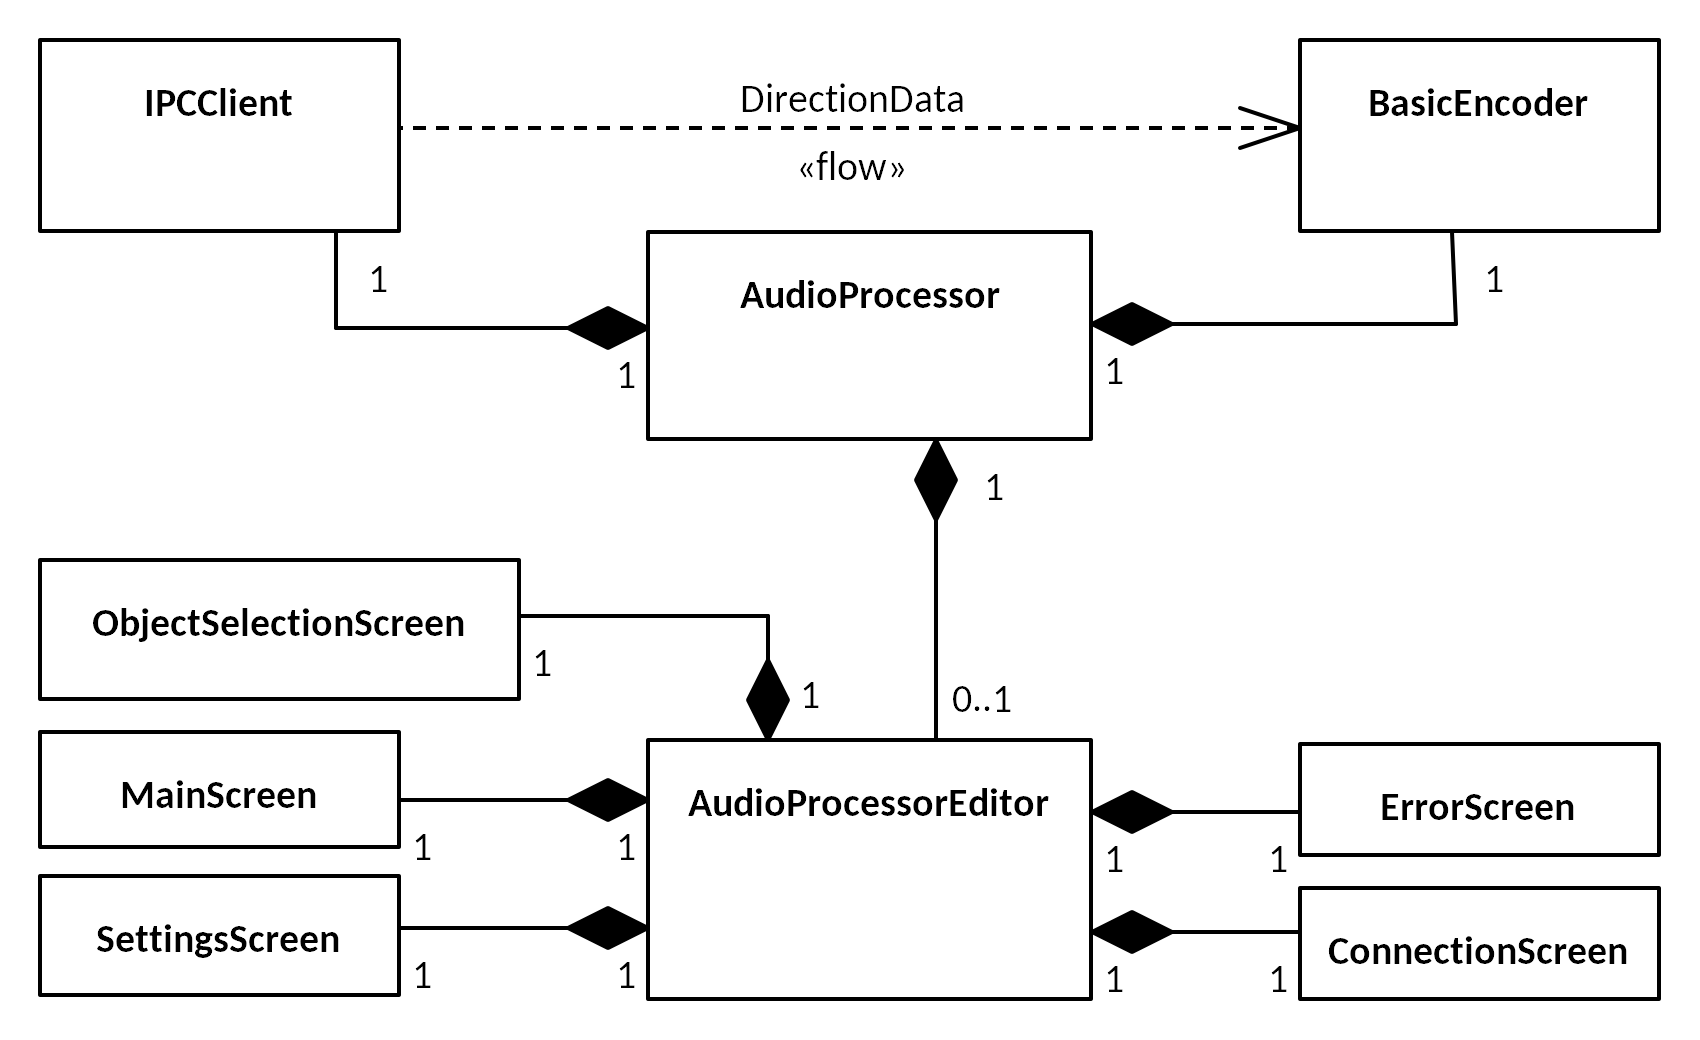
\includegraphics[width=0.7\textwidth]{images/implementation/vst_simplified_class_diagram.png}
    \caption{Simplified class diagram for the Ambilink VST plugin. (This diagram only includes the most important classes, and is not by any means an exhaustive representation of the whole architecture.)
    Image courtesy of the author. \label{fig:vst_class_diagram}}
\end{figure}

Figure \ref{fig:vst_class_diagram} shows the high level structure of the Ambilink VST plugin.
The \cppinline{AudioProcessor} class holds instances of the \cppinline{IPCClient} and the \cppinline{BasicEncoder} classes.
The \cppinline{IPCClient} class handles communication with the Blender plugin, and the \cppinline{BasicEncoder} class performs the 
ambisonic panning. (The two classes have no knowledge of each other, the direction data is passed through the \cppinline{AudioProcessor} class.)

\subsection{IPC}
The \cppinline{IPCClient} class is implemented as a state machine. The states and transitions can be seen in figure \ref{fig:ipc_state_machine}.
The ``Error'' state and corresponding transitions, as well as transitions to the ``Disconnected`` state are omitted from the diagram to keep it comprehensible.
Whenever connection to the Blender plugin is lost (e.g. if Blender is closed, or the server is stopped by the user), 
the IPC client transitions to the ``Disconnected'' state, regardless of what state it was in previously.
Whenever an exception not caused by connection loss occurs in any of the states, the VST transitions to a special ``Error'' state. 
The GUI then displays an error message, and a button allowing to transition back to the ``Disconnected'' state.
(The plugin will then automatically transition to either ``Connected'' or ``Subscribed'', depending on what state it was in before the error occurred.)
While the users should hopefully never be able to experience the error screen by themselves,
having such a fail-safe allows the plugin to recover gracefully from situations that would have otherwise lead to a crash.

\begin{figure}%[!ht]
    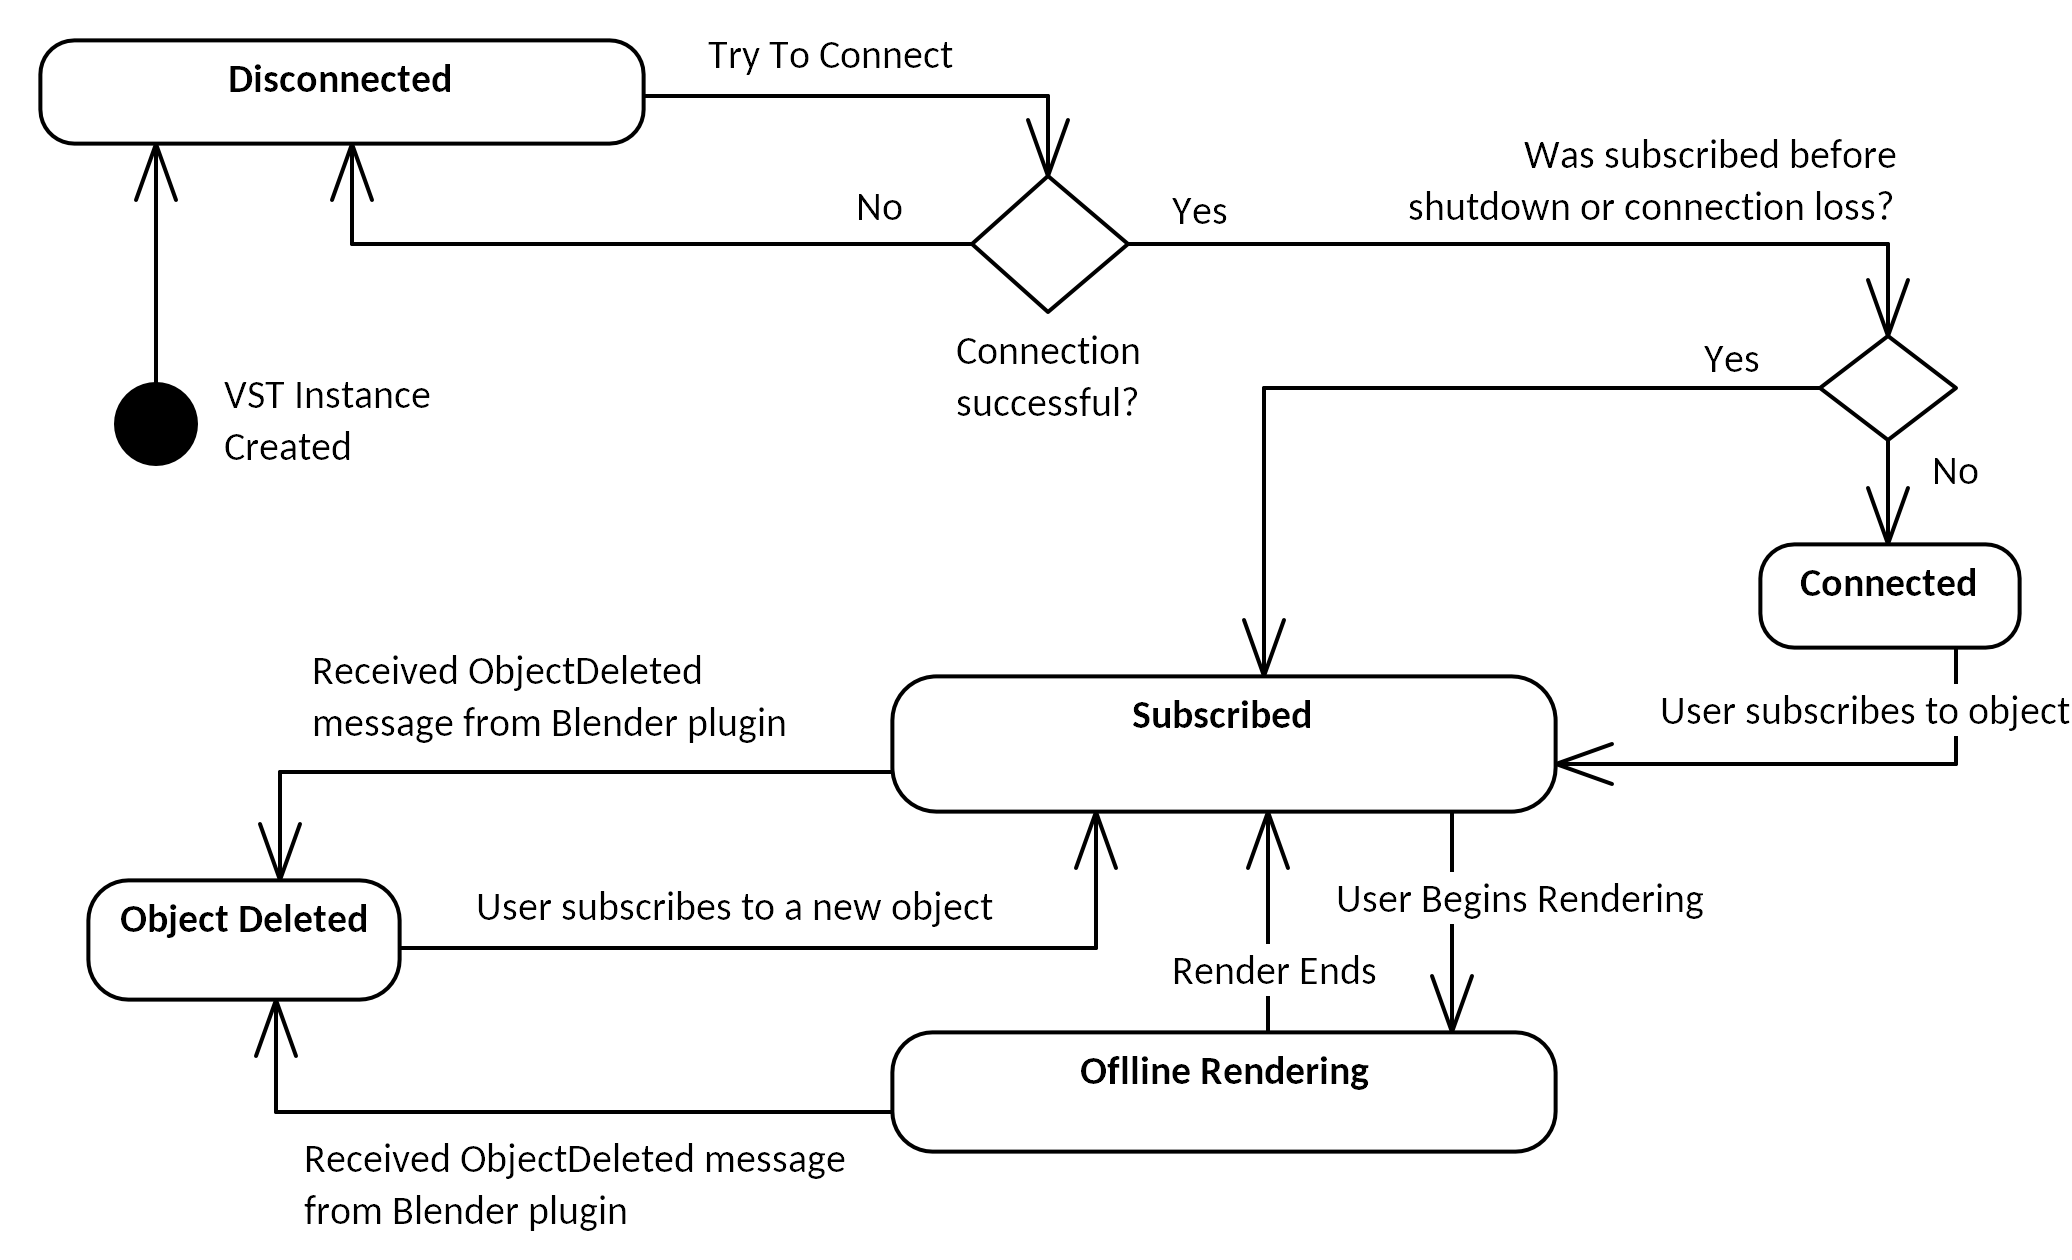
\includegraphics[width=0.8\textwidth]{images/implementation/vst_ipc_state_machine.png}
    \centering
    \caption{State machine diagram describing the way IPC is implemented on the VST side.
             Image courtesy of the author. \label{fig:ipc_state_machine}}
\end{figure}

\cppinline{IPCClient} spawns two threads, one for each communication pattern - a requestor thread, and a subscriber thread.
Each class implementing a state has specific functions to send requests to the Blender plugin,
and to receive messages published using Pub/Sub.
These functions are called by the main \cppinline{IPCClient} class from the respective threads.

To reduce coupling, other parts of the plugin control IPC using a custom event system.
For example, the \cppinline{ObjectSelectionScreen} class can instruct the \cppinline{IPCClient} to subscribe to an object by publishing an event.
The event is passed to \cppinline{IPCClient} through the \cppinline{AudioProcessorEditor} and \cppinline{AudioProcessor} classes.
This is done to further reduce coupling and allow some events to be ``intercepted'' and acted upon by classes other than the \cppinline{IPCClient}.

Once an event reaches the \cppinline{IPCClient}, it is added to a lock-free queue implemented using atomic variables (The implementation used in Ambilink is inspired by Fabian Renn-Giles's \nobreak{farbot} library \cite{farbot_repo}.).
Thread-safety is required since the events are added and removed by different threads; the lock-free implementation reduces overhead of posting an event.
\cppinline{IPCClient}'s requestor thread consumes events from the queue, and passes them to the currently active state,
the state class can then perform any required action, e.g. sending requests or initiating a transition to a different IPC state.

Upon transitioning to the ``Subscribed'' state, the subscriber thread is spawned and begins consuming messages published by the Blender plugin.
When an \cppinline{OBJ_POSITION_UPDATED} message is received, it calculates the direction and distance to the object from the camera space coordinates, 
and updates the values of atomic variables, that are then read by the audio thread and passed to the encoder. 

\subsection{Multithreading in a real-time context}
Real-time audio processing is quite different from most problems usually encountered by programmers.
In case of VST plugins, the host software manages the high-priority threads used for audio processing.
The plugin's processing function (\cppinline{AudioProcessor::processBlock()} in case of plugins using JUCE) is repeatedly called from the audio thread,
each time with new audio and/or MIDI data for the plugin to process. \cite{juce_audioprocessor_doc}
The main caveat is that this callback has to always finish in time. Any delay, even if it occurs extremely rarely
will result in audible artifacts in the audio. \cite{rt_101_talk_part_1}\cite{locks_in_real_time_blog_post}

For example, if the sample rate of the host software is $44.1kHz$, and the size of the audio buffers passed to the plugin is 128 samples,
then the \cppinline{AudioProcessor::processBlock()} function must take less than $(1/44100)*128 = 0.0029s$ to execute, which is just under $3ms$\footnote{
    The sample rate can be significantly higher (usually in the range of $44.1-192 kHz$). Buffer sizes can go down to 32, or even 16 samples. (Speaking from personal experience using DAWs and working with audio.)
}. \cite{locks_in_real_time_blog_post}
This limitation rules out any operation that doesn't have a reliable time limit.
Examples of such operations include accessing files, any form of network communication (or IPC), and, importantly,
using mutex-based thread synchronisation techniques.
Practically any call to a function not implemented by the program should be treated as not real-time safe
unless the documentation explicitly states otherwise. \cite{rt_101_talk_part_1} 
All of these operations can of course be performed on other threads, but if the data needs to be passed to the audio thread
it has to be done without using traditional synchronisation primitives.
Thankfully, even when using locks is out of the question, race conditions can be avoided with good design and some tricks.
In simpler cases, using an atomic value that is modified by one thread and read by another is sufficient, 
but various thread-safe lock-free data structures, such as single consumer single producer FIFO queues can also be implemented (mostly by clever use of atomic variables).
For further information on real-time audio programming I would recommend the two part talk by Fabian Renn-Giles and Dave Rowland \cite{rt_101_talk_part_1}\cite{rt_101_talk_part_2},
which I used as the main source of information on this topic.
Fabian Renn-Giles's open source farbot library \cite{farbot_repo} which implements many real-time safe data structures may also be of interest to the reader.

In case of Ambilink, the data used in the audio processing callback has to be passed from the Pub/Sub thread.
Since the data is small\footnote{
    A struct of two \cppinline{float}s for the direction and a single \cppinline{float} for the distance.
}, 
this is realised using a pair of atomic variables that are ensured to be lock-free
by static assertions (\cppinline{std::atomic<T>::is_always_lock_free}). The atomic variables are stored by 
\cppinline{IPCClient} and read by the audio thread whenever required.
In offline rendering mode, however, a lock is utilised so the audio thread can get access 
to the instance of the \cppinline{OfflineRendering} state\footnote{
    The mutex is only used to prevent the \cppinline{IPCClient} from switching to a different state,
    which would result in destruction of the \cppinline{OfflineRendering} object.
    Synchronisation between the Req/Rep thread and the audio thread,
    once the audio thread does gets access to the state, is performed using 
    atomic variables.
}. This does not really pose a problem since the audio 
is not played back in real time in this case and because locking the mutex
will be uncontested unless a communication error occurs and IPC needs to switch to a different state.
It is however undebatable that this part of the implementation could benefit from optimisation in the future.

\subsection{Encoder}
As mentioned previously, \cppinline{BasicEncoder} is the class that handles ambisonic panning of the incoming audio. 
On each invocation of the \cppinline{AudioProcessor::processBlock()} function, the encoder's 
direction and distance parameters are updated. In real-time mode, the latest value processed by the \cppinline{IPCClient} is used.
In offline rendering mode, direction and location at the respective time in the animation are used.

\begin{listing}[ht]
\begin{minted}{python}
def encode(input_buffer, ambisonic_order, direction, distance, 
           max_distance, distance_attenuation_curve)
{
    curr_sh_coefficients = 
        calc_spherical_harmonic_coefficients(ambisonic_order, direction)
    gain = gain_from_distance(distance, max_distance, 
                              distance_attenuation_curve)

    encoded_with_prev_direction =
        matmult(_prev_sh_coefficients, input_buffer.with_gain(_prev_gain))
    encoded_with_curr_direction = 
        matmult(curr_sh_coefficients, input_buffer.with_gain(gain))

    _prev_sh_coefficients = curr_sh_coefficients
    _prev_gain = gain

    return crossfade(encoded_with_prev_direction,
                     encoded_with_curr_direction)
}
\end{minted}
\caption{The encoding algorithm used by the \cppinline{BasicEncoder} class in pseudocode. Member variables are prefixed with underscores.}
\label{pseudocode:encoding_algo}
\end{listing}

A version of the encoding algorithm used by Ambilink written in pseudocode can be seen in listing \ref{pseudocode:encoding_algo}.
(The actual C++ code is too verbose to be included as a listing.) 
The ambisonic-encoded buffers are produced by matrix multiplication of the input audio sample vector $\bm{x}$, and 
the vector of spherical harmonic coefficients $\bm{s}$ that is 
calculated using the \cppinline{getRSH_recur()} function from the Spatial Audio Framework library (\cite{saf_repo}) based on the 
direction received from \cppinline{IPCClient}. For first-order ambisonics, this would look as follows:
\begin{equation}
    \bm{s}^T\bm{x} = 
    \begin{bmatrix} w\\ x\\  y\\ z\\ \end{bmatrix}
    \begin{bmatrix} x_1& x_2 & \cdots &x_n\\ \end{bmatrix} =
    \begin{bmatrix}
        W_{1}  & W_{2}  & \cdots & W_{n} \\
        X_{1}  & X_{2}  & \cdots & X_{n} \\
        Y_{1}  & Y_{2}  & \cdots & Y_{n} \\
    \end{bmatrix}
\end{equation}

The same calculation is performed twice, with the spherical harmonic coefficients and gains from the previous and current method calls,
and the resulting buffers are then cross-faded to avoid audible artifacts in the audio when the direction or distance changes rapidly.

\subsection{Limitations} \label{subsection:vst_limitations}
Due to limitations of the VST3 format, Ambilink only supports ambisonics up to fifth order.
The VST3 interface requires the plugin's main output bus\footnote{In this context, the word ``bus'' refers to a set of audio channels.}
to conform to one of the output channel sets explicitly specified by Steinberg
\footnote{In the VST3 interface, these are referred to as ``speaker arrangements''. The current definitions can be found here \cite{vst3_doc_speaker_arrangement}, 
but the page is likely to be updated as new versions of the SDK are released.}. 
The VST3 interface still only officially supports ambisonic channel sets up to third order, but
JUCE manages to support fourth and fifth order ambisonics, potentially using some undocumented behaviour of the VST3 interface.
Curiously, the previous version of the interface - VST2, supported so-called ``discrete'' 
layouts for a plugin's main output, which basically allowed to use any number of output channels without explicitly 
labeling what CBA or SBA format the plugin's output conforms to. 
Discussion regarding the issue on Steinberg's forums (\cite{vst3_hoa_steinberg_forums}) has started as early as April 2018 and continues as of February 2023.
Development team members have been intermittently discussing possible solutions and proposals in the thread, 
but the issue has not been resolved as of February 2023.

\section{Blender add-on}
The Ambilink blender add-on is written in Python (as all Blender add-ons are) and supports Blender version 3.4.1 - the latest one at the time of development.
In contrast to the VST, the Blender add-on only uses one external module - pynng, the previously mentioned Python wrapper for the NNG library.

\subsection{Software architecture}

As can be seen in figure \ref{fig:blender_addon_class_diagram}, the architecture of the Blender add-on is simpler than that of the VST plugin. 
There are two main classes - \cppinline{IPCServer} and \cppinline{ObjectInfoManager}.
The \cppinline{IPCServer} class handles all details of the IPC protocol - decoding incoming requests, correctly structuring and encoding reply data, etc.
It holds an instance of \cppinline{ObjectInfoManager} that takes care of the ``business logic'' of the add-on, but has no knowledge of the IPC protocol itself.
\cppinline{ObjectInfoManager}'s responsibilities include keeping track of all objects with at least one subscriber,
informing the \cppinline{IPCClient} class (via callbacks) whenever the objects are renamed or deleted, 
providing object locations and other information about the Blender scene, such as animation length and FPS.

\begin{figure}%[!ht]
    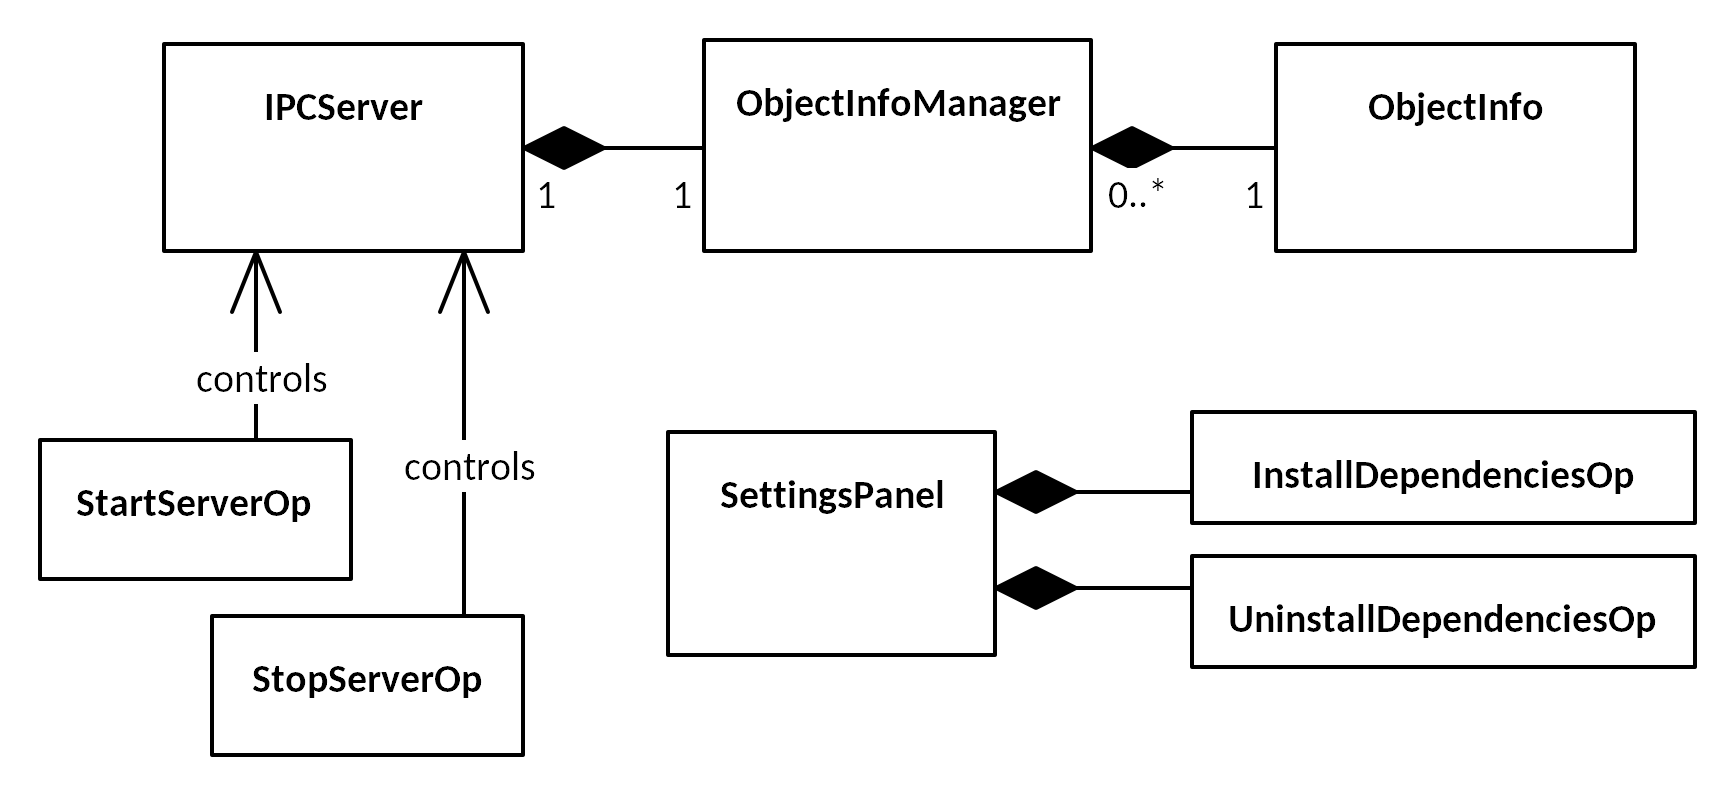
\includegraphics[width=0.8\textwidth]{images/implementation/blender_add_on_class_diagram.png}
    \centering
    \caption{Simplified class diagram for the Ambilink Blender add-on. (For the sake of conciseness, the diagram does not include some helper classes, e.g. custom exception types.)
             Image courtesy of the author. \label{fig:blender_addon_class_diagram}}
\end{figure}

\subsection{Multithreading considerations}

The add-on needs to continuously reply to requests and publish messages for subscribed VST instances. 
Ideally this would be done in a separate thread, but Blender's Python scripting implementation is not thread safe.
Thus, all access to Blender data needs to be performed on the thread the add-on is launched from, which also happens to be 
the GUI thread\footnote{This means that long operations performed by the add-on will result in Blender's GUI being unresponsive.}.
While spawning another thread and passing commands using a thread-safe queue or a similar mechanism is possible, 
such an approach didn't make much sense for Ambilink, especially for the initial implementation. 
Because the majority of IPC commands require accessing Blender data, only a limited number of operations, such as encoding and decoding message data,
could have been performed in a separate thread, so the performance improvement (if any) 
provided by a multithreaded implementation wouldn't have been significant enough to justify the added complexity.

Instead of using a separate thread for IPC communication, messages are sent and received by a method that is called 
on the main thread multiple times per second. This is achieved using the \cppinline{StartServerOp} (``Start Server For Ambilink VST'') modal operator.
\footnote{Modal operators can continue running in the background after being invoked by the user.}
Once it is invoked by the user, it creates an \cppinline{IPCServer} instance and schedules a timer that calls it's \pythoninline{serve} method multiple times per second.
(The update frequency can be configured via add-on settings, the default is 30 Hz.)
On each invocation, the \pythoninline{serve} method replies to all pending requests sent by VST instances and publishes updates for any registered
objects\footnote{I will sometimes refer to objects with at least one subscribing VST instance as ``registered objects'' for the sake of conciseness.}.

\subsection{Overcoming Blender API limitations} \label{subsection:blender_api_fun}

Blender's Python API is realised via the \pythoninline{bpy} Python module that is accessible to add-ons and scripts.
It allows to access and modify most aspects of the 3D scene including the names and locations of objects,
so, at first glance, keeping track of this data should be simple.
Objects in the scene can easily be accessed by their name, e.g. \pythoninline{bpy.context.scene.objects['Name']}.
However, as mentioned previously, the name of the object is not a viable unique identifier for Ambilink's use case
since an object can be renamed after a subscription is established, and an Ambilink-specific identifier (Ambilink ID) is used instead.

\begin{listing}
    \begin{minted}{python}
    def get_scene_objects():
        return bpy.context.scene.objects

    def lookup_by_name():
        return get_scene_objects().get(TEST_OBJ_NAME)

    def lookup_by_prop():
        for obj in get_scene_objects():
            if obj.get(TEST_PROP_NAME) == DESIRED_PROP_VALUE:
                return obj
    \end{minted}
\caption{Functions used to compare performance of looking up Blender objects by name and by value of a custom property.
         Test results are presented in table \ref{table:blender_obj_lookup_test_results}.}
\label{python:obj_lookup_test_funcs}
\end{listing}

\begin{table}
\centering
{\setlength{\extrarowheight}{0.2em}%
\begin{tabular}{ |m{\textwidth-29em}|m{13em}|m{12em}| } 
\hline
                                & A single object has the custom property assigned &  All objects have the custom property assigned \\
\hline
\pythoninline{lookup_by_name()} & 20.42s                                           & 19.76s \\
\hline
\pythoninline{lookup_by_prop()} & 96.88s                                           & 128.85s \\
\hline
Performance decrease            & 4.74x                                            & 6.51x \\
\hline
\end{tabular}}
\vspace{1em}
\caption{Test results for performance of Blender object lookup by name and by value of a custom property
         using lookup functions from code listing \ref{python:obj_lookup_test_funcs}.
         The times in the table correspond to the total time it took to find a specific Blender object
         $100000$ times. The tests were performed using the \pythoninline{timeit} Python module.
         \label{table:blender_obj_lookup_test_results}}
\end{table}


Unfortunately, as evident from the test results presented in table \ref{table:blender_obj_lookup_test_results}, 
finding an object by it's Ambilink ID is much slower than using the object's name.
The times in the table correspond to the total time it took to lookup a specific Blender object $100000$ times 
using the \pythoninline{lookup_by_name()} and \pythoninline{lookup_by_prop()} functions (code listing \ref{python:obj_lookup_test_funcs}).
There was a total of $2380$ objects in the Blender scene, and the same object,
located at index $1871$ in the \pythoninline{bpy.context.scene.objects} collection, was being looked up each time.
Two tests have been performed. In the first test, there was only one object in the scene that had the custom property set.
In the second test, all objects in the scene had the custom property set, but only one of them had it set to \pythoninline{DESIRED_PROP_VALUE}.
The Python script and the Blender project used to perform the tests can be found in the attached media.
The results show that lookup using the value of a custom property takes roughly 5 times longer
than lookup by name. This can be explained by the fact that getting an object by it's name is handled 
directly by Blender's C++ implementation, and finding an object
by the value of a custom property requires iterating all objects in the scene from Python code.
\footnote{I have initially expected Blender's implementation to use a hashmap for looking up objects by name,
but the \cppinline{RNA_property_collection_lookup_string} 
function defined in the \cppinline{rna_access.c} file (\cite{blender_git_rna_lookup_string})
seems to simply iterate over all items in the collection. (Which seems to be more than fast enough.)}

In an ideal case, the Blender add-on would avoid the need to constantly search the list of all objects
in the scene by storing a reference\footnote{
Variables in Python ``are simply names that refer to objects'' (\cite{python_docs_references}), meaning that 
assigning an object to a variable always results in storing a reference to that object and never in copying the object itself.
} to the actual Python object\footnote{
    There may be some confusion between objects as in object-oriented programming, and 3D objects in the Blender scene.
    I will try to avoid the ambiguity by always referring to the first kind as ``Python objects''.
} returned by Blender's API.
The situation is however complicated by the fact that references to Blender data 
returned by \pythoninline{bpy} can be invalidated under some circumstances.
The most common case when this occurs is whenever the Undo/Redo functionality is used.

To maximise performance, Ambilink uses a combination of storing object references returned by 
\pythoninline{bpy}, lookup by name, and lookup by Ambilink ID.
When a VST instance subscribes to a previously unregistered object, an Ambilink ID is generated
and stored in Blender's object data as a custom property.
The Python object (reference) returned by Blender, the object's name, and the assigned Ambilink ID are stored
in an instance of the \cppinline{ObjectInfo} class. The name stored by the Ambilink add-on is kept up to date 
even if the object is renamed by subscribing to updates of it's ``name'' property 
using the \pythoninline{bpy.msgbus.subscribe_rna} function.
\begin{samepage}
Whenever a property of a Blender object needs to be accessed, the following steps are taken:
\begin{enumerate}
    \item Try to access the object through the stored reference.
    \item If the previous step fails, try to find the object by name.
    \item If both previous steps fail, try to find the object by Ambilink ID.
\end{enumerate}
\end{samepage}
If all of the steps listed above fail, the Blender object is treated as deleted and an \cppinline{OBJ_DELETED} message is published.
Additionally, the add-on registers handlers that are called by Blender on Undo/Redo operations.
This allows to keep the stored references valid and avoid the need to lookup objects by name or Ambilink ID most of the time.

While fairly complicated, the described approach minimises the time it takes to access properties of registered objects
by using the fastest approach under most circumstances and only falling back to the slower options if needed.
The slowest option - lookup by Ambilink ID - should only ever be used in the Undo/Redo handlers, when the operation
being undone or redone is renaming an object, and, even in that case, only for one object, because multiple 
objects can't be renamed as part of one Undo or Redo operation.
In all other cases, Blender should invoke the object name update handler
registered by each \cppinline{ObjectInfo} instance, keeping the name stored by the Ambilink add-on up to date,
and ensuring lookup by name succeeds.

\subsection{Limitations}\label{subsec:blender_addon_limitations}
Using custom properties is the only way to attach custom data to Blender objects. 
For most use cases, this approach works great. The only caveat is, when a Blender object is duplicated 
it's custom properties are duplicated as well. This is a problem for Ambilink since duplicating an object with 
at least one subscribing VST instance results in a Blender scene containing two objects with identical Ambilink IDs. 
This results in what the C++ standard would call undefined behaviour.

The current version of Ambilink does not attempt to solve this in any way, but a potential future workaround 
would be to override all of Blender's built-in operators that allow the user to duplicate an object 
resulting in duplication of custom properties. Unfortunately, there are at least four such operators.
Two of them
are specific to object duplication (\pythoninline{bpy.ops.duplicate_move} and \pythoninline{bpy.ops.duplicate_move_linked}), 
but the same result can be achieved by copying and pasting an object 
either from the 3D viewport (\pythoninline{bpy.ops.view3d.pastebuffer}) 
or the object list (\pythoninline{bpy.ops.outliner.id_paste}).
